
\subsubsection{UC27-Selezione modalità di divisione del conto}
\begin{figure}[h] 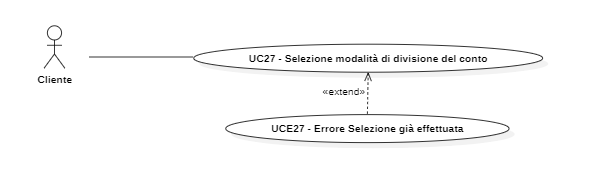
\includegraphics[scale=1]{uc27.png} \end{figure}
\begin{itemize}
\item \textbf{Attore principale:} Cliente.
\item \textbf{Precondizioni:} Il cliente deve avere:
  \begin{itemize}
    \item Una prenotazione accettata dal ristoratore;
    \item Limite temporale di modifica degli ordini deve essere stato superato;
    \item Deve essere stata fatta almeno una ordinazione;
    \item Deve essere stata scelta la modalità di divisione del conto.
  \end{itemize}
\item \textbf{Postcondizioni:} Il conto viene diviso a seconda della modalità scelta.
\item \textbf{Scenario principale:}
\begin{enumerate}
    \item Il cliente clicca sulla selezione della modalità di divisione del conto;
    \item Il cliente clicca sceglie se pagamento equo o proporzionale;
    \item Il cliente viene reindirizzato alla visualizzazione della singola prenotazione.
\end{enumerate}
\end{itemize}

\subsubsection{UCE27-Errore selezione già effettuata}
\begin{itemize}
\item \textbf{Attore principale:} Cliente.
\item \textbf{Descrizione:} Uno solo dei clienti può effettuare la selezione della modalità di divisione del conto.
  il primo che preme, sceglie per tutti.
\item \textbf{Scenario alternativo:}
\begin{enumerate}
    \item Il cliente clicca sulla selezione della modalità di divisione del conto;
    \item Il sistema mostra un messaggio di errore;
    \item Il cliente viene reindirizzato visualizzazione del conto di ogni cliente.
\end{enumerate}
\end{itemize}

\subsubsection{UC28-Pagamento in app}
\begin{figure}[h] 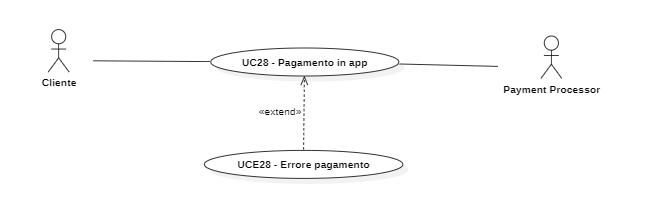
\includegraphics[scale=1]{uc28.png} \end{figure}
\begin{itemize}
\item \textbf{Attore principale:} Cliente.
\item \textbf{Attore secondario:} Processore di pagamenti.
\item \textbf{Precondizioni:} Il cliente deve avere:
  \begin{itemize}
    \item Una prenotazione accettata dal ristoratore;
    \item Limite temporale di modifica degli ordini deve essere stato superato;
    \item Deve essere stata fatta almeno una ordinazione;
    \item Deve essere stata scelta la modalità di divisione del conto.
  \end{itemize}
\item \textbf{Postcondizioni:} Il sistema segna il cliente / le ordinazioni come pagati.
\item \textbf{Scenario principale:}
\begin{enumerate}
    \item Il cliente seleziona la prenotazione che vuole pagare;
    \item Il cliente clicca sul tasto paga;
    \item Il sistema mostra un form con un menù a tendina chiedente il metodo di pagamento
      (Carta di credito, carta di debito, Paypal, etc);
    \item Il cliente clicca sul tipo desiderato;
    \item Il sistema crea un richiesta di pagamento tramite il metodo desiderato e
      apre una scheda dove il cliente può pagare;
    \item Il cliente paga;
    \item Il sistema riceve la conferma del pagamento;
    \item Il sitema reindirizza il cliente alla pagina di visualizzazione della singola prenotazione;
    \item Il cliente visualizza la pagina della singola prenotazione con ciò che ha pagato segnato come tale;
\end{enumerate}
    \item \textbf{Estensioni:}
        \begin{itemize}
                \item UCE28-Errore di pagamento.
        \end{itemize}
\end{itemize}

\subsubsection{UCE28-Errore di pagamento}
\begin{itemize}
\item \textbf{Descrizione: } Il processore di pagamento ha dato un errore.
\item \textbf{Scenario alternativo:}
\begin{enumerate}
    \item Al momento di ricezione della conferma viene ottenuto un errore;
    \item Il sistema comunica che il pagamento non è andato a buon fine;
    \item Il cliente visualizza il form della selezione del tipo di pagamento desiderato.
\end{enumerate}
\end{itemize}

\subsubsection{UC29-Inserimento di feedback e recensioni} % analizzare più in dettaglio
\begin{figure}[h] 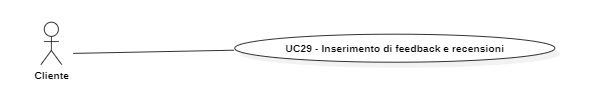
\includegraphics[scale=1]{uc29.png} \end{figure}
\begin{itemize}
\item \textbf{Attore principale:} Cliente.
\item \textbf{Precondizioni:}
  \being{itemize}
    \item Il cliente sta visualizando una prenotazione accettata;
    \item La prenotazione è stata pagata.
  \end{itemize}
\item \textbf{Postcondizioni:} La recensione è stata salvata nella lista di recensioni del ristorante.
\item \textbf{Scenario principale:}
\begin{enumerate}
    \item Il cliente clicca sul tasto per lasciare una recensione;
    \item Il sistema mostra un form contente tre voti da una a cinque stelle, rispettivamente per:
  \begin{itemize}
    \item Menù;
    \item Servizio;
    \item Prezzo.
  \end{itemize}
      Segue poi un campo di testo;
    \item Il cliente può riempire i tre voti (obbligatori) e il campo di testo (facoltativo);
    \item Il cliente fa il submit del form;
    \item Il sistema reindirizza alla pagina del ristorante dove è possibile vedere la propria recensione.
\end{enumerate}
\end{itemize}

\pagebreak
\subsubsection{UC30-Visualizzazione notifica cambio stato prenotazione}
\begin{figure}[h] 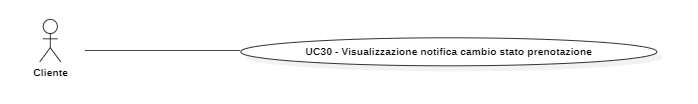
\includegraphics[scale=1]{uc30.png} \end{figure}
\begin{itemize}
\item \textbf{Attore principale:} Cliente.
\item \textbf{Attore secondario:} Ristoratore.
\item \textbf{Precondizioni:} Il cliente ha una prenotazione in attesa di essere accettata.
\item \textbf{Postcondizioni:} Il cliente visualizza una notifica con il nuovo stato della prenotazione
\item \textbf{Scenario principale:}
\begin{enumerate}
    \item Il ristoratore accetta o rifiuta la prenotazione;
    \item Al cliente compare una notifica contenente il nuovo stato della prenotazione (accettata o rifiutata).
\end{enumerate}
\end{itemize}

\subsubsection{UC31-Visualizzazione notifica ricezione messaggio in chat}
\begin{figure}[h] 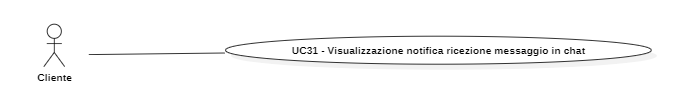
\includegraphics[scale=1]{uc31.png} \end{figure}
\begin{itemize}
\item \textbf{Attore principale:} Cliente.
\item \textbf{Precondizioni:}
\begin{itemize}
    \item Il cliente ha avviato la chat con il ristoratore (si veda UC49);
    \item Il ristoratore ha inviato un messaggio al cliente (si veda UC50.1).
\end{itemize}
\item \textbf{Postcondizioni:} Il cliente visualizza una notifica relativa alla ricezione di un messaggio in chat.
\item \textbf{Scenario principale:}
\begin{enumerate}
    \item Il sistema vede che è stato inviato un messaggio dal ristoratore;
    \item Il sistema invia al cliente una notifica relativa al messaggio;
    \item Il cliente visualizza la notifica relativa al messaggio.
\end{enumerate}
\end{itemize}

\pagebreak
\subsubsection{UC32-Visualizzazione notifica accettazione invito da parte di altri utenti}
\begin{figure}[h] 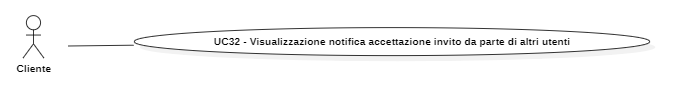
\includegraphics[scale=1]{uc32.png} \end{figure}
\begin{itemize}
\item \textbf{Attore principale:} Cliente.
\item \textbf{Precondizioni:} Il cliente ha una prenotazione accetata e ha condiviso il link di invito tramite terze parti.
\item \textbf{Postcondizioni:} Il cliente visualizza una notifica con il nome del profilo di chi ha accettato l'invito.
\item \textbf{Scenario principale:}
\begin{enumerate}
    \item L'utente che ha ricevuto il link di invito seleziona un profilo;
    \item Il sistema aggiunge il profilo selezionato alla prenotazione;
    \item Il sistema notifica il cliente dell'accettazione di invito;
    \item Al cliente mittente compare una notifica contentente il nuovo profilo aggiuntosi alla prenotazione.
\end{enumerate}
\end{itemize}
